\documentclass[mgr, shortabstract]{iithesis}

\usepackage[utf8]{inputenc}
\usepackage{amsmath}
\usepackage{minted}
\usepackage{listings}
\usepackage{graphicx}

%%%%% DANE DO STRONY TYTUŁOWEJ
\polishtitle    {Polski tytuł}
\englishtitle   {English title}
%\polishabstract {\ldots}
%\englishabstract{\ldots}
\author         {Maksymilian Debeściak}
% w przypadku kilku promotorow, lub koniecznosci podania ich afiliacji, linie
% w ponizszym poleceniu mozna zlamac poleceniem \fmlinebreak
\advisor        {dr Jan Kowalski}
%\date          {}                     % Data zlozenia pracy

\polishabstract {Polskie streszczenie}
\englishabstract {Angielskie streszczenie}

% Dane do oswiadczenia o autorskim wykonaniu
%\transcriptnum {}                     % Numer indeksu
%\advisorgen    {dr. Jana Kowalskiego} % Nazwisko promotora w dopelniaczu
%%%%%

%%%%% WLASNE DODATKOWE PAKIETY
%
%\usepackage{graphicx,listings,amsmath,amssymb,amsthm,amsfonts,tikz}
%

%%%%% WŁASNE DEFINICJE I POLECENIA
%
%\theoremstyle{definition} \newtheorem{definition}{Definition}[chapter]
%\theoremstyle{remark} \newtheorem{remark}[definition]{Observation}
%\theoremstyle{plain} \newtheorem{theorem}[definition]{Theorem}
%\theoremstyle{plain} \newtheorem{lemma}[definition]{Lemma}
%\renewcommand \qedsymbol {\ensuremath{\square}}
% ...
%%%%%

\newmintedfile[swiftcode]{swift}{
  fontsize=\footnotesize
}

\newmintedfile[objccode]{objc}{
  fontsize=\footnotesize
}

\newcommand{\todo}[1]{
  \textit{\textbf{TODO: }#1}
}

\newcommand{\ang}[1]{ang. \textit{#1}}

\newcommand{\swiftlisting}[2]{
    \swiftcode{src/#1.swift}
    \begin{listing}[ht]
      \caption{#2}
      \label{l:#1}
    \end{listing}
}

\newcommand{\objclisting}[2]{
    \objccode{src/#1.m}
    \begin{listing}[ht]
      \caption{#2}
      \label{l:#1}
    \end{listing}
}

\begin{document}

%%%%% POCZĄTEK ZASADNICZEGO TEKSTU PRACY

\chapter{Wstęp}
\label{ch:wstep}

...

\chapter{Podobieństwa do innych języków programowania}
\label{ch:podobienstwa_do_innych}

\section{Podstawowe cechy}
\label{s:podstawowe_cechy}

Swift to wieloparadygmatowy język programowania łączący pomysły znane z innych popularnych języków, takich jak: Objective-C, C\#, Rust, Haskell czy Ruby. Podobnie jak C\#, pozwala na tworzenie struktur (typów wartościowych), klas (typów referencyjnych) i typów wyliczeniowych. Wspiera również dziedziczenie (ale nie wielokrotne), definiowanie protokołów (odpowiednik interfejsów z C\# czy Java) oraz polimorfizm parametryczny (typy generyczne), nie pozwala natomiast na definiowanie klas abstrakcyjnych, zachęcając tym samym programistów do szerokiego stosowania interfejsów.

\section{Typy generyczne}
\label{s:typy_generyczne}

Swift wspiera dwie podstawowe koncepcje generyczności:
\begin{itemize}
  \item klasy, struktury, typy wyliczeniowe oraz funkcje z parametrami typu (ang. \textit{generics})
  \item protokoły z powiązanymi typami (ang. \textit{associated types})
\end{itemize}

Klasy (struktury, funkcje) ze zmiennymi typu to pomysł dobrze znany z większości popularnych języków programowania obiektowego, takich jak C\# czy Java. W momencie definiowania klasy programista ma możliwość zdefiniowania zmiennych przebiegających przestrzeń typów używanych w definiowanej klasie. Dodatkowo Swift oferuje kilka bardziej zaawansowanych mechanizmów związanych ze zmiennymi typu:

\begin{itemize}
  \item możliwość dodania ograniczeń na typy, po których przebiega zmienna, np. zmienna może być tylko typem implementującym dany protokół lub dziedziczącym po danej klasie
  \item automatyczna inferencja typów paremetrów generycznych
  \item możliwość nadawania aliasów funkcjom i typom generycznym
\end{itemize}

Przykład użycia typów generycznych ilustruje Listing \ref{l:2_generics_and_inheritance}.

\swiftlisting
    {2_generics_and_inheritance}
    {Przykład klasy generycznej i klasy pochodnej w Swift}

W odróżnieniu od klas, struktur i funkcji, protokoły nie wspierają generycznych paremetrów typu. Zamiast tego, protokoły posiadają mechanizm typów powiązanych (\ang{associated types}), wzorowany na znanym np. ze Scali mechanizmie abstrakcyjnych pól typu (\ang{abstract type members}). Pozwala on na zdefiniowanie w protokole zmiennej typu, która zostanie ukonkretniona dopiero przez klasę implementującą dany protokół. Główną zaletą tego rozwiązania jest ukrycie typu podstawionego pod zmienną typu przed programistą używającym klasy implementującej dany protokół - typ podstawiony pod zmienną jest częścią implementacji i nie musi być jawnie podawany podczas tworzenie obiektu implementującego protokół. Przykład użycia protokołu z parametrami typu prezentuje Listing \ref{l:2_associated_types}.

\swiftlisting
    {2_associated_types}
    {Przykład protokołu z typem powiązanym w Swift}

\section{Typy wartościowe i referencyjne}
\label{s:typy_wartosciowe_i_refrencyjne}

Podobnie jak w języku C\#, typy w Swifcie można podzielić na dwie grupy:

\begin{itemize}
    \item typy wartościowe (\ang{value types})
    \item typy referencyjne (\ang{reference types})
\end{itemize}

Typy wartościowe to typy, które tworzą nowe instancje obiektów podczas przypisywania do zmiennej lub przekazywania do funkcji. Innymi słowy, każda instancja posiada swoją własną kopię danych, obiekty takie nie dzielą ze sobą stanu, przez co są łatwiejsze w zrozumieniu i bezpieczniejsze przy pracy z wieloma wątkami. Jeśli zmienna typu wartościowego zostanie zadeklarowana jako stała, cały obiekt, łącznie ze wszystkimi polami nie może zostać zmieniony. Typami wartościowymi w Swifcie są:

\begin{itemize}
    \item struktury
    \item typy wyliczeniowe
    \item krotki
\end{itemize}

Typy referencyjne to typy, których obiekty dzielą pomiędzy sobą te same dane, a podczas przypisywania lub przekazywania do funkcji tworzona jest tylko nowa referencja do tych samych danych. Zmienne typu referencyjnego zadeklarowane jako stałe zapewniają jedynie stałość referencji, jednak dane przypisane do zmiennej mogą być bez dowolnie zmieniane. Typami referencyjnymi w Swifcie są tylko klasy.

\swiftlisting
    {2_class_struct_protocol_enum}
    {Przykładowe definicje podstwowych obiektów w Swift: struktury, klasy, protokołu i typu wyliczeniowego}

\section{Domknięcia jako typy pierwszoklasowe}
\label{s:domkniecia_jako_typy_pierwszoklasowe}

Podobnie jak w językach funkcyjnych i w większości nowoczesnych języków programowania obiektowego, domknięcia w Swifcie są typem pierwszoklasowym (\ang{first-class citizen}), tzn:

\begin{itemize}
    \item mogą być przechowywane w zmiennych i stanowić elementy struktur danych
    \item mogą być podawane jako parametry wywołania funkcji i metod
    \item mogą byc zwracane przez funkcje i metody
\end{itemize}

\swiftlisting{2_closures}{Przykład użycia domknięcia w Swift}

\section{Leniwość}
\label{s:leniwosc}

Swift jest domyślnie językiem z ewaluacją gorliwą, autorzy zaimplementowali jednak dwa rozwiązania pozwalające w podstawowym stopniu na wspieranie leniwych obliczeń. Po pierwsze, w Swifcie, podobnie jak w C\#, istnieje możliwość leniwej inicjalizacji obiektów. O ile jednak w C\# mechanizm ten polega na użyciu klasy $Lazy$ z biblioteki standardowej, o tyle w Swifcie jest on zaszyty w samym języku - służy do tego słowo kluczowe $lazy$. Drugim rozwiązaniem są leniwe struktury danych, których implementacja opera się na znanych również z języka C\# czy Java generatorach.

\swiftlisting
    {2_laziness}
    {Przykład deklaracji leniwej zmiennej i leniwej sekwencji w Swift}

\section{Elementy zaczerpnięte z języków funkcyjnych}
\label{s:element_zaczerpniete_z_jezykow_funkcyjnych}

Pomimo tego, że Swift był projektowany głównie jako język programowania obiektowego, jego twórcy skupili dużą część swojej uwagi na elementach powiązanych z programowaniem funkcyjnym, które mogłyby pomóc programistom pisać bezpieczniejszy i bardziej czytelny kod obiektowy. Najważniejsze z nich to:

\begin{itemize}
    \item Typy wyliczeniowe z wartościami powiązanymi (\ang{associated values}), które wprowadzają do Swifta koncept podobny do konstruktorów typów z Haskella. Dzięki tym strukturom danych, programista może w funkcyjny deklarować nowe typy (zob. Listing \ref{l:2_enum_with_associated_value}).

    \swiftlisting
        {2_enum_with_associated_value}
        {Implementacja drzewa binarnego w Swift}

    \item Dzięki zwięzłej i eleganckiej składni oraz potraktowaniu domknięć na równi klasami i stukturami, Swift oferuje bardzo dobre wsparcie dla funkcji wyższego rzędu. Funkcje wyższego rzędu są też często używane w bibliotece standardowej, np. kolekcje danych posiadają najczęściej używane funkcje służące do manipulowania nimi, takie jak \texttt{filter}, \texttt{map}, \texttt{reduce} czy \texttt{flatMap}.

    \item Autorzy Swifta postawili bardzo duży nacisk na niemutowalność (\todo{lepsze słowo?}) danych, co przejawia się w całej składni języka, np. dostępne jest słowo odrębne słowo kluczowe \texttt{let} służące do deklarowania stałych, parametry przekazywane do funkcji są domyślnie stałymi, użycie typów wartościowych jest preferowane nad użyciem klas (również w bibliotece standardowej) itp.

    \item Swift posiada zaawansowany mechanizm \textit{pattern matchingu}, który można wykorzystać do dopasowywania typów wyliczeniowych, krotek i wyrażeń. Tak jak w wielu językach funkcyjnych, \textit{pattern matching} w Swifcie jest wyczerpujący (\ang{exhaustive}), co oznacza, że każda wartość, która może pojawić się podczas dopasowywania musi zostać obsłużona.

    \item Aby uniknąć problemów z wartością \texttt{nil}, w języku Swift każda zmienna musi zostać zainicializowana już w momencie deklaracji. Jeśli programista chce celowo stworzyć zmienną mogącą przyjmować wartość \texttt{nil}, powinien użyć typu \texttt{Optional<T>}, który w swojej konstrukcji jest bardzo podobny do monady \texttt{Maybe} znanej z Haskella. Istnieje nawet mechanizm zwany \textit{optional chaning}, który zachowuje się tak, jak operacja \texttt{>>=} dla monady \texttt{Maybe}.

    \swiftlisting
        {2_optional}
        {Typ \texttt{Optional} i mechanizm \textit{optional chaining}}

\end{itemize}

\section{Zwięzłość składni}
\label{s:zwiezlosc_skladni}

Jednym z największych problemów podczas programowania w Objective-C była słaba czytelność kodu i bardzo rozwlekła składnia. Dlatego podczas projektowania Swifta iżynierowie Apple mocno wzorowali się na językach znanych ze swojej zwięzłości i łatwości czytania, takich jak Python czy Ruby. Zrezygnowano z plików nagłówkowych, wprowadzono dużo cukru syntaktycznego dla najcześciej stosowanych konstrukcji (jak np. operator \texttt{T?} dla typu \texttt{Optional<T>}), wprowadzono domyślną inferencję typów. Rysunek \ref{f:keynote} pokazuje różnice pomiędzy kodem napisanym w Objective-C, a takim samym kodem w Swift.

\begin{figure}[ht]
\makebox[\textwidth][c]{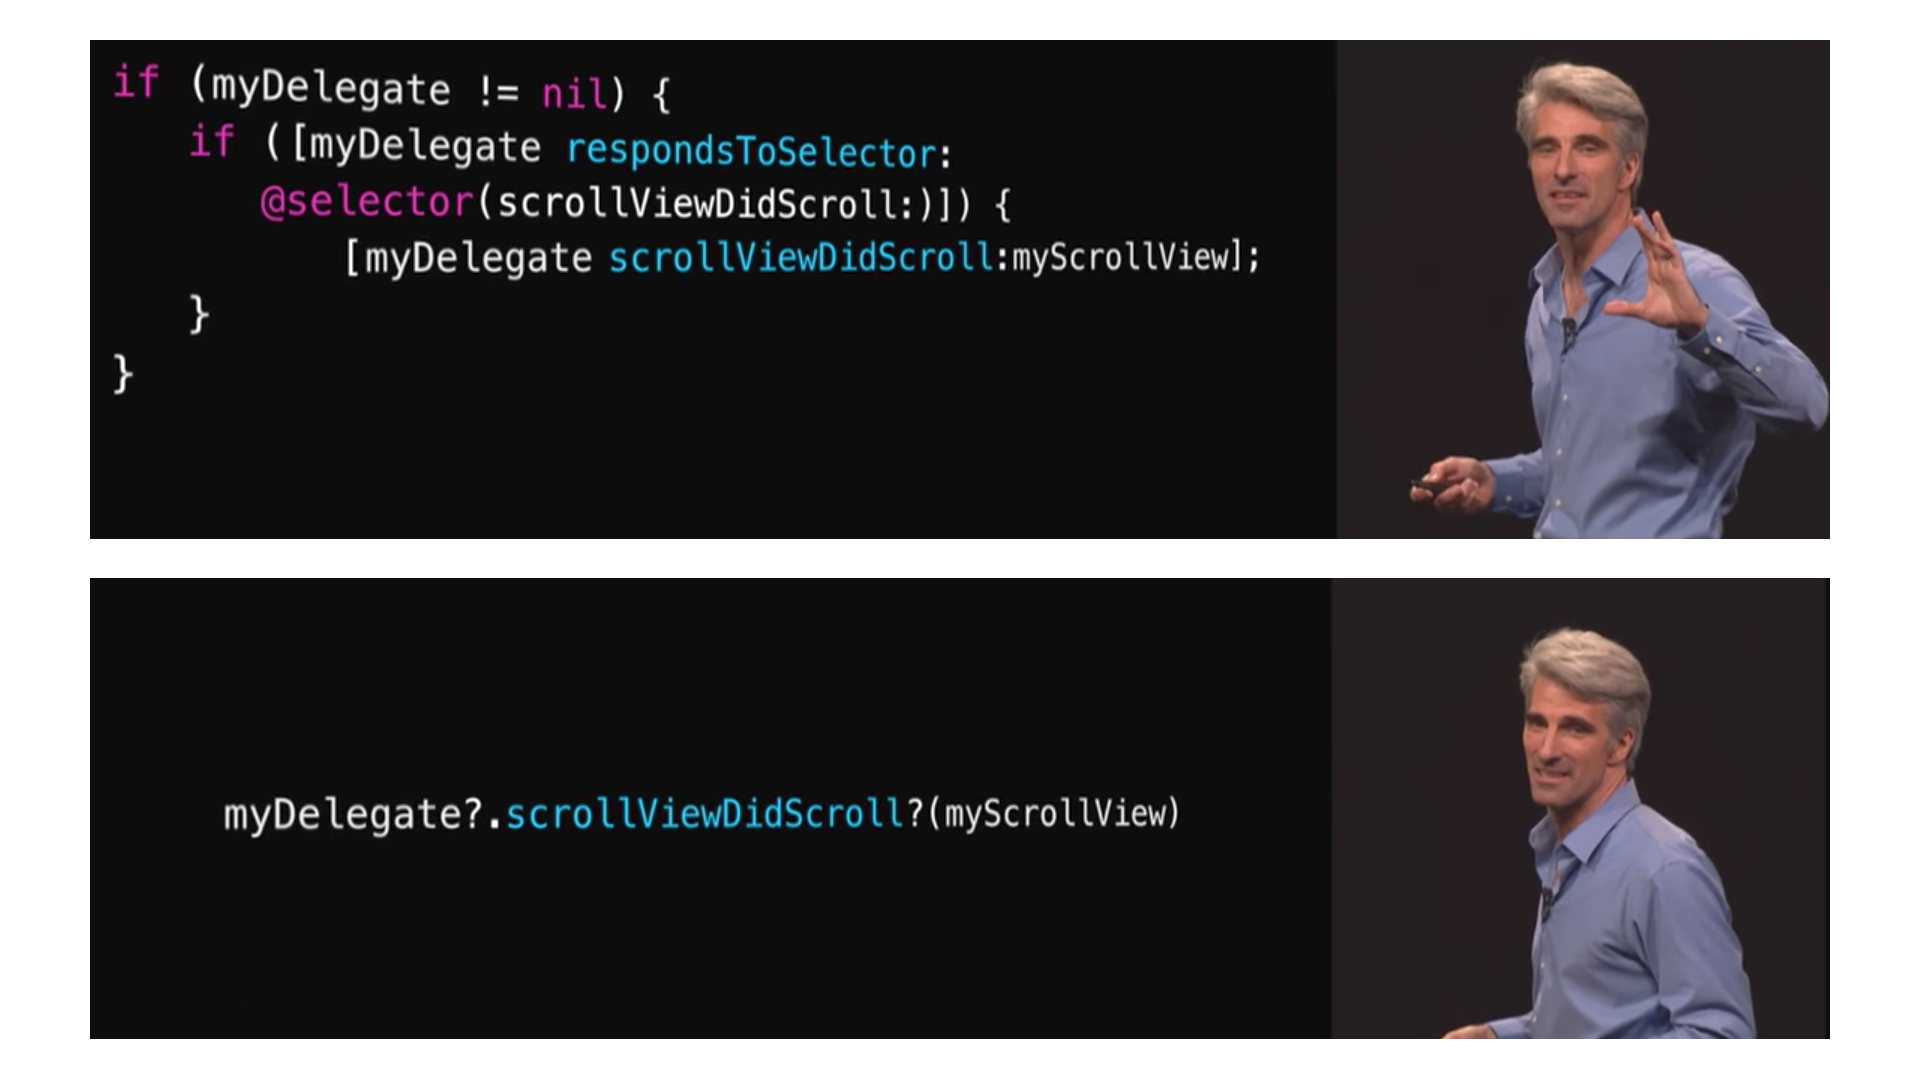
\includegraphics[width=1.2\textwidth]{images/Keynote.png}}
\caption{Craig Federighi wskazuje różnice pomiędzy czytelnością kodu Objective-C (na górze) i Swift (na dole). \textit{WWDC Keynote 2014}}
\label{f:keynote}
\end{figure}

\section{Rozszerzenia typów}
\label{s:rozszerzenia_typow}

Jedną z rzadziej spotykanych w językach statycznie typowanych językach programowania funkcjonalności jest możliwość rozszerzania istniejących już typów. Co prawda już w Objective-C programista miał moliwość stworzenia kategorii (\ang{category}), ale pozwalała ona tylko na dodawanie nowych funkcji, nie można było natomiast definiować nowych właściwości, konstruktorów ani typów zagnieżdżonych. Dlatego w Swifcie zotały zaimplementowane rozszerzenia (\ang{extensions}), które pozwalają na:

\begin{itemize}
    \item dodawanie nowych właściwości obliczanych (\ang{computed properties})
    \item definiowanie nowych metod instancji i metdo typu
    \item definiowanie nowych inicializatorów
    \item definiowanie i używanie typów zagnieżdżonych
    \item implementowanie metod protokołów
\end{itemize}

\swiftlisting{2_extension}{Przykład rozszerzenia w Swift}

\chapter{Podobieństwa i różnice pomiędzy Swiftem i Objective-C}

\todo{Dwa słowa o samym Objective-C?}

\section{Podobieństwa}

\subsection{Swift i Objective-C jako języki programowania obiektowego}

Zarówno Swift, jak i Objective-C są głównie językami programowania  obiektowego. Oba języki pozwalają na definiowanie własnych typów (klasy i typy wyliczeniowe w Objective-C, struktury, klasy oraz typy wyliczeniowe w Swifcie), wspierają dziedziczenie i polimorfizm. Dzięki modyfikatorom dostępu umożliwiają również enkapsulację implementacji i opisywanie zachowań za pomocą abstrakcyjnych typów danych (protokoły w Objective-C, interfejsy w Swifcie).

\objclisting{3_objective_c_example}{Przykład kodu obiektowego w Objective-C}

\swiftlisting{3_swift_example}{Analogiczny kod napisany w Swifcie}

\subsection{Zarządzanie pamięcią}

W początkowych wersjach systemu OSX i iOS zarządzanie pamięcią było w pełni manualne - co prawda obiekty (a raczej wskaźniki do nich) posiadały liczniki referencji, jednak programista musiał sam zadbać o zarządzanie tymi licznikami. Przełom nastąpił w roku 2011, kiedy to do Objective-C zostało dodane automatyczne zliczanie referencji (\ang{automatic reference counting}, w skrócie: ARC).

Automatyczne zliczanie referencji to jedna z najprostszych metod zarządzania pamięcią, odciążajaca programistę z obowiązku jawnego inkrementowania i dekrementowania liczników referencji. Użycie ARC w Objective-C powoduje wygenerowanie kodu, który zwiększa licznik referencji w momencie, gdy nowa referencja do obiektu zostaje utworzona (np. inicjalizacja, przypisanie, przekazania obiektu w parametrze) oraz zmniejsza go, w momencie usunięcia referencji. Dzięki temu programista nie musi manualnie używać funkcji \texttt{retain} i \texttt{release}, jak to miało miejsce w poprzednich wersjach Objective-C. Pozwala to na wyłapanie wielu błędów, takich jak: wycieki pamięci, wielokrotne zwalnianie pamięci czy odwoływanie się do wcześniej zwolnionej pamięci. Jednocześnie, użycie ARC nie wprowadza niedeterminizmu, co ma miejsce w przypadku użycia automatycznego odśmiecania pamięci (\ang{garbage collector}) oraz ma znikomy wpływ na wydajność działania aplikacji.

ARC jest również metodą zarządzania pamięcią zaimplementowaną w Swifcie. Główną różnicą jest jednak sposób implementacji. W Objective-C, ARC jest rozszerzeniem języka, operającym się głównie na preprocesorze i generowaniu kodu odpowiedzialnego za zliczanie referencji. W Swifcie natomiast, ARC jest jego podstawową cechą, posiadającą odrębną składnię i wparcie ze strony środowiska uruchomieniowego.

\subsection{Biblioteki}

Jedną z cech, dla której Swifta tak szybko zdobywa popularność jest możliwość wywoływania kodu Objective-C z poziomu kodu swiftowego i na odwrót (\ang{interoperability}). Z tego względu prawie wszystkie biblioteki standardowe posiadają bardzo podobne interfejsy i są dostępne w obu językach. Oba języki posiadają też możliwość wywoływania kodu pisanego w języku C, dlatego też wiele z bardziej zaawansowanych bibliotek, jak np. CoreAudio czy GLKit (\todo{źródło}).

\section{Różnice}

\subsection{Składnia}

Objective-C to język, którego początki sięgają pierwszej połowy lat 80. Z tego powodu, niektóre jego cechy są w tym momencie uważane w środowisku developerów systemów iOS i OSX, za przestarzałe i niewygodne. Mając te cechy na uwadze, inżynierowie Apple opracowali nowy język z uproszczoną składnią i wieloma udogodnieniami pozwalającymi programistom w krótszym czasie pisać kod, który będzie czytelniejszy i łatwiejszy w utrzymaniu.

Pierwszym z udogodnień zaimplementowanych Swifta jest inferencja typów. W Objective-C każdy typ zmiennej musiał zostać jawnie napisany, co szczególnie w przypadku długich, złożonych typów (np. zawierających parametry generyczne) mogło być mocno uciążliwe. Kompilator Swifta natomiast stara się wywnioskować tak wiele informacji o typach, ile jest w stanie.

Po drugie, sama składnia języka jest dużo bardziej zwięzła i czytelna. w Swifcie usunięto konieczność pisania nawiasów przy warunkach intrukcji warunkowych i pętli, dodano możliwość oddzielania kolejnych intrukcji poprzez znak nowej linii (nie ma potrzeby pisania znaku średnika na końcu linii), zaimplementowano dużo prosztszą obsługą stringów, dodano dużo czytelniejszą składnię dla funkcji wyższego rzędu, zrezygnowano z plików nagłówkowych (modyfikatory dostępu definiuje się podobnie jak w Javie czy C\#). Dodatkowo, najczęściej używane struktury składniowe otrzymały prostsze formy w postaci cukru syntaktycznego, np:

\begin{itemize}
    \item definicja zmiennej \mintinline{swift}{var x: Int?} jest tożsama z \mintinline{swift}{var x: Optional<Int>}
    \item konstrukcja \texttt{if let} jest cukrem syntaktycznym dla sprawdzania, czy wartość typu \mintinline{swift}{Optional<T>} nie jest nilem
    \item Swift 2.2 wprowadził cukier syntaktyczny dla selektorów (obiektów zawierających informacje pozwalające wywoływać na obiektach funkcje w runtime)
    \item pattern matching dla typów wyliczeniowych i krotek to bardzo mocno rozwinięty cukier syntaktyczny dla instrukcji warunkowych dla tych typów
\end{itemize}

\subsection{Zarządzanie pamięcią}

Pomimo, że zarówno Objective-C, jak i Swift korzystają z automatycznego zliczania referencji, jego implementacja jest diametralnie różna. W Objective-C ARC został dodany jako jedno z rozszerzeń języka C, jego implementacja bazuje głównie na wykorzystaniu makr i preprocesora, który automatycznie wstawia kod odpowiedzialny za zarządzanie licznikiem referencji. W Swifcie natomiast, ARC jest podstawowym elementem języka posiadającym odrębną składnię i słowa kluczowe.

\subsection{System typów}

Oba omawiane języki są językami statyczni typowanymi, jest jednak pomiędzy nimi kilka istotnych różnic:

\begin{itemize}

    \item w Swifcie w zasadzie nie występuje niejawne rzutowanie typów. Każde (nawet najprostsze, jak rzutowanie z typu całkowitoliczbowego na zmiennoprzeciknowy) musi być jawnie napisane przez programistę. W Objective-C zasady rzutowania zostały odziedziczone z języka C i są w zasadzie takie same.
    \item sposób wywoływania metod został zaczerpnięty z języka Smalltalk i odbywa się poprzez wysyłanie wiadomości (\ang{message}) pomiędzy obiektami. Z tego względu rozwiązywanie, którą funkcję należy wywołać dzieje się w metodzie \mintinline{objc}{objc_msgSend} w trakcie działania programu.
    \item w Objective-C istnieje klasa \mintinline{objc}{NSObject}, która jest superklasą dla wszystkich innych klas. Swift nie posiada takiej superklasy, została ona zastąpiona protokołem \mintinline{swift}{AnyObject}.

\end{itemize}

\subsection{Bezpieczeństwo}

Jednym z podstawowych założeń przyjętych przy tworzeniu Swifta było stworzenie języka, który będzie chronił programistę przed najczęstszymi błędami popełnianymi podczas pisania kodu. Najważniejsze mechanizmy służące temu celowi to:

\begin{itemize}
    \item typ \mintinline{swift}{Optional<T>} - typ ten chroni przed wszelkimi błędami związanymi z wartością \texttt{null}
    \item konieczność inicjalizacji obiektu - każdy obiekt musi zostać zainicjalizowany w trakcie zadeklarowania referencji, co zapobiega problemom z dostępem do jeszcze nie zainicjalizowanej pamięci
    \item generyczne struktury danych - Objective-C nie posiadało typów generycznych, przez co struktury danych mogły przechowywać wartości różnych typów, co z kolei powodowało konieczność sprawdzania typów. W Swifcie struktury są silnie typowane i homogeniczne
    \item domyślna niemutowalność - w Swifcie istnieje wiele miejsc, gdzie obiekty są domyślnie niemutowalne, np przy przekazywaniu do funkcji
    \item preferowanie typów wartościowych nad referencyjne - typy wartościowe zapobiegają zmianom jednego obiektu z wielu miejsc, przez co czytelność i łatwość zrozumienia kodu jest dużo większa
    \item automatyczne sprawdzanie przekroczenia zakresu liczb całkowitych
    \item zmiany w składni, takie jak: obowiązkowe nawiasy \texttt{\{...\}} dla ciał funkcji warunkowych i pętl, obsługa wszystkich możliwych wartości dla typów wyliczeniowych, konieczność zwrócenia wartości w fukcjach, które deklarują zwracany typ, brak instrukcji \texttt{goto} itp.
\end{itemize}


%%%%% BIBLIOGRAFIA

%\begin{thebibliography}{1}
%\bibitem{example} \ldots
%\end{thebibliography}

\end{document}
